\documentclass[a4paper,14pt]{extarticle}

\usepackage[a4paper,top=20mm,bottom=20mm,left=30mm,right=10mm]{geometry}
\usepackage[T1,T2A]{fontenc}
\usepackage[utf8]{inputenc}
\usepackage[russian]{babel}
\usepackage{indentfirst}
\usepackage{titlesec}
\usepackage{graphicx}
\usepackage{verbatim}
\usepackage{fancyvrb}

\renewcommand{\baselinestretch}{1.3}
\titleformat{\section}{\normalsize\bfseries}{\thesection}{1em}{}
\titleformat{\subsection}{\normalsize\bfseries}{\thesection}{1em}{}
\setlength{\parindent}{12.5mm}

\begin{document}

  \newpage\thispagestyle{empty}
  \begin{center}
    \MakeUppercase{
      Министерство науки и высшего образования Российской Федерации\\
      Федеральное государственное бюджетное образовательное учреждение высшего образования\\
      <<Вятский Государственный Университет>>\\
    }
    Институт математики и информационных систем\\
    Факультет автоматики и вычислительной техники\\
    Кафедра электронных вычислительных машин
  \end{center}
  \vfill

  \begin{center}
    Отчет по лабораторной работе №3\\
    по дисциплине\\
    <<Программирование>>\\
  \end{center}
  \vfill

  \noindent
  \begin{tabular}{ll}
    Выполнил студент гр. ИВТб-1301-05-00 \hspace{5mm} &
    \rule[-1mm]{25mm}{0.10mm}\,/Макаров С.А./\\
    
    Руководитель зав. кафедры ЭВМ & \rule[-1mm]{25mm}{0.10mm}\,/Долженкова М.Л./\\
  \end{tabular}

  \vfill
  \begin{center}
    Киров 2024
  \end{center}

  \newpage
  \section*{Цель}
  Цель лабораторной работы: освоить синтаксис построения процедур и функций, изучить способы передачи данных в подпрограммы, получить навыки организации минимального пользовательского интерфейса.

  \section*{Задание}
  Реализовать программу вычисления площади фигуры, ограниченной кривой
  $2 * x^3 -2 * x^2 + 0 * x + 16$ и осью OX (в положительной части по оси OY). Вычисление определенного интеграла должно выполняться численно, с применением метода левых прямоугольников. Пределы интегрирования вводятся пользователем. Взаимодействие с пользователем должно осуществляться посредством case-меню. Требуется реализовать возможность оценки погрешности полученного результата. Необходимо использовать процедуры и функции там, где это целесообразно.

  \section*{Решение}
  \begin{figure}[h]
    \centering
    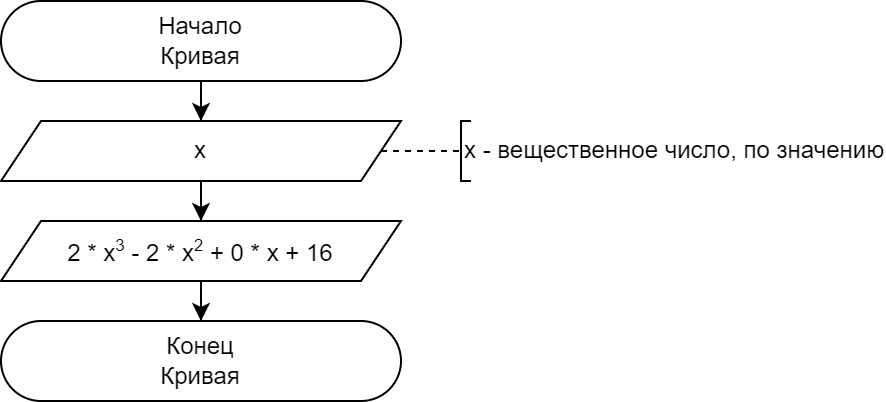
\includegraphics[width=0.6\linewidth]{images/s-1}
  \end{figure}
  \begin{center}
    Рисунок 1 – Подпрограмма <<Кривая>>
  \end{center}

  \pagebreak
  \begin{figure}[h]
    \centering
    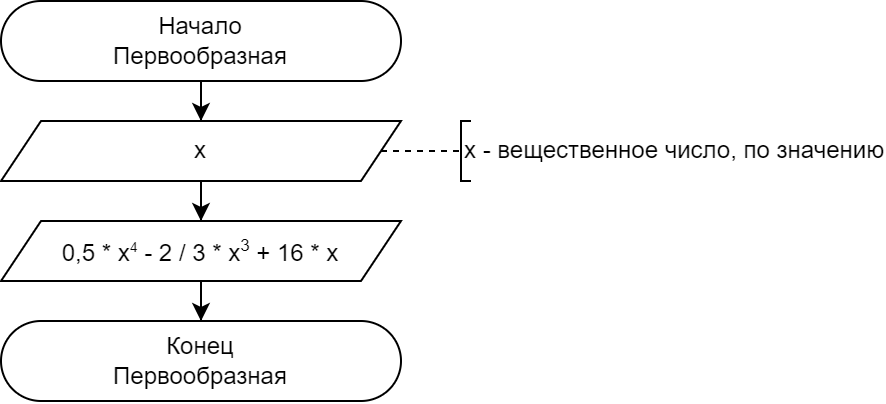
\includegraphics[width=0.6\linewidth]{images/s-2}
  \end{figure}
  \begin{center}
    Рисунок 2 – Подпрограмма <<Первообразная>>
  \end{center}

  \begin{figure}[h]
    \centering
    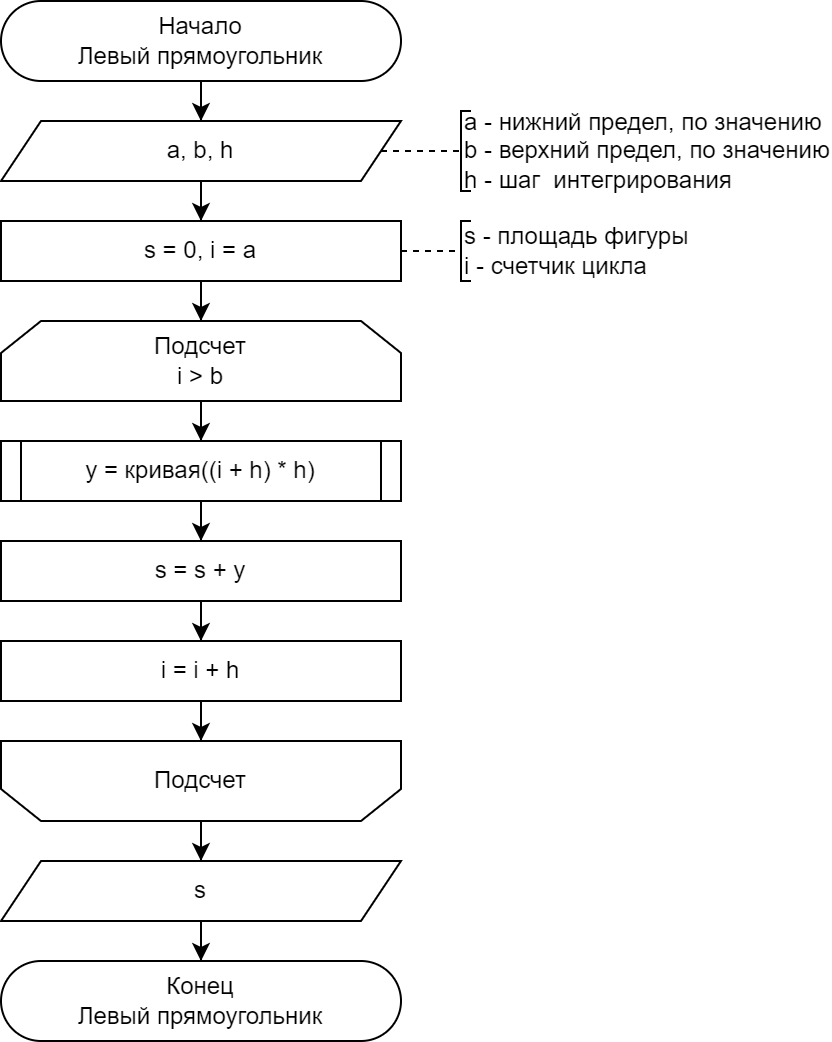
\includegraphics[width=0.6\linewidth]{images/s-4}
  \end{figure}
  \begin{center}
    Рисунок 3 – Подпрограмма <<Левый прямоугольник>>
  \end{center}

  \pagebreak
  \begin{figure}[h]
    \centering
    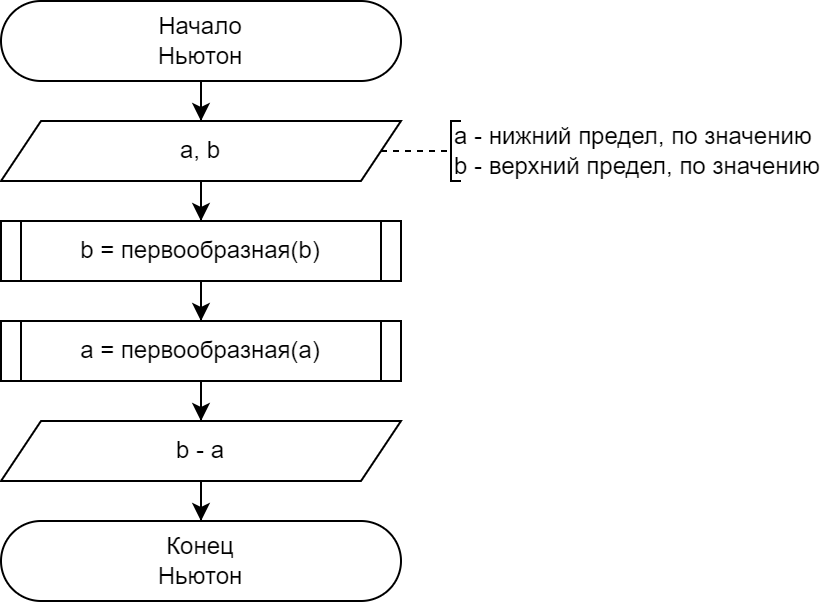
\includegraphics[width=0.6\linewidth]{images/s-3}
  \end{figure}
  \begin{center}
    Рисунок 4 – Подпрограмма <<Ньютон>>
  \end{center}

  \begin{figure}[h]
    \centering
    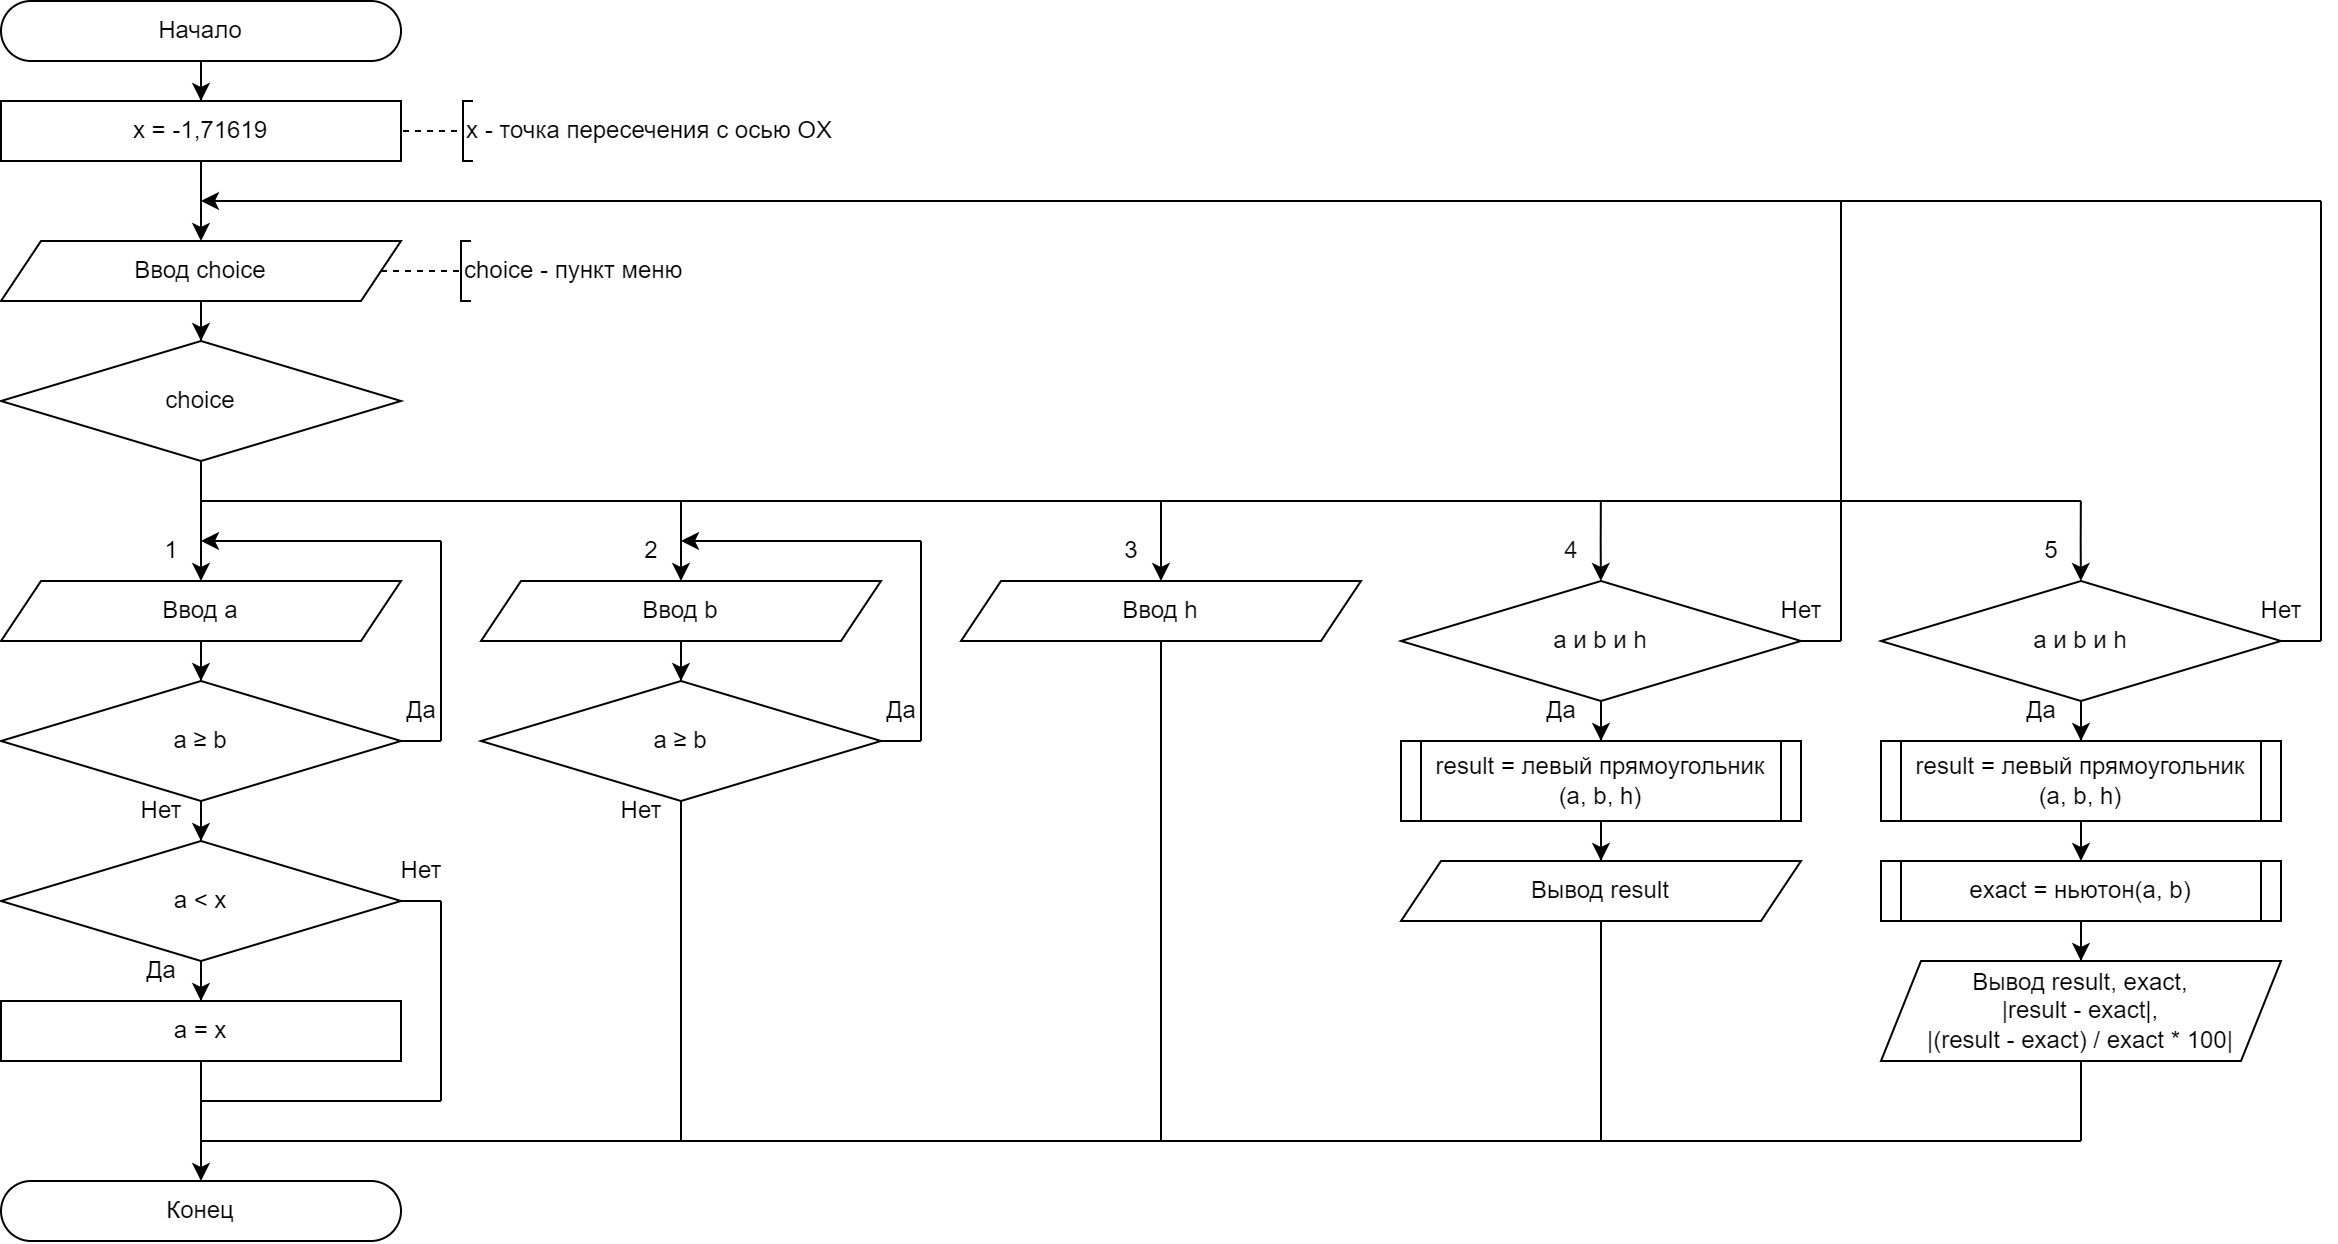
\includegraphics[width=1\linewidth]{images/s-5}
  \end{figure}
  \begin{center}
    Рисунок 5 – Схема алгоритма программы
  \end{center}

  \newpage
  \begin{Verbatim}[tabsize=2]
#include <stdio.h>
#include <stdlib.h>
#include <math.h>
#define X -1.71619

float curve(float x) {
  return 2 * pow(x, 3) - 2 * pow(x, 2) + 0 * x + 16;
}

float antiderivative(float x) {
  return 0.5 * pow(x, 4) - 2.0 / 3.0 * pow(x, 3) + 16 * x;
}

float calc_newton(float a, float b) {
  return antiderivative(b) - antiderivative(a);
}

float left_rect(float a, float b, float h) {
  float s = 0.0;
  
  for (float i = a; i < b; i = i + h) {
    s += curve(i + h) * h;
  }
  
  return s;
}

void print_menu() {
  printf("\033[0d\033[2J");
  printf("1. Ввод нижнего предела\n");
  printf("2. Ввод верхнего предела\n");
  printf("3. Ввод шага интегрирования\n");
  printf("4. Рассчет интеграла\n");
  printf("5. Рассчет погрешности\n");
}

void print_input(int *choice) {
  printf(">  ");
  scanf("%d", &*choice);
}

int main() {
  int choice, is_a = 0, is_b = 0, is_h = 0;
  float a, b, h;
  
  print_menu();
  print_input(&choice);
  
  while(1)
  {
    switch (choice)
    {
      case 1:
        print_menu();
        printf("Нижний предел: ");
        scanf("%f", &a);
        
        if (is_b) while (a >= b) {
          printf("Введите корректный нижний предел: ");
          scanf("%f", &a);
        }
        if (a < X) a = X;
        is_a = 1;
        print_input(&choice);
        break;
      
      case 2:
        print_menu();
        printf("Верхний предел: ");
        scanf("%f", &b);
        
        if (is_a) while (a >= b) {
          printf("Введите корректный верхний предел: ");
          scanf("%f", &b);
        }
        is_b = 1;
        print_input(&choice);
        break;
        
        case 3:
        print_menu();
        printf("Шаг интегрирования: ");
        scanf("%f", &h), is_h = 1;
        print_input(&choice);
        break;
      
      case 4:
        print_menu();
        if (is_a && is_b && is_h) {
          printf("Площадь: %.2f\n", left_rect(a, b, h));
        } else {
          printf("Не введены пределы или шаг интегрирования\n");
        }
        print_input(&choice);
        break;
      
      case 5:
        print_menu();
        if (is_a && is_b && is_h) {
          printf("Метод левых прямоугольников: %.2f\n", 
              left_rect(a, b, h));
          printf("Метод Ньютона-Лейбница:      
              %.2f\n", calc_newton(a, b));
          printf("Абсолютная погрешность:      %.2f\n", 
              fabs(left_rect(a, b, h) - calc_newton(a, b)));
          printf("Относительная погрешность:   %.2f%%\n",
              fabs((left_rect(a, b, h) - calc_newton(a, b)) /
              calc_newton(a, b) * 100));
        } else {
          printf("Не введены пределы или шаг интегрирования\n");
        }
        print_input(&choice);
        break;
      
      default:
        print_menu();
        print_input(&choice);
        break;
    }
  }
  return 0;
}
  \end{Verbatim}

  \section*{Вывод}
  В ходе выполнения лабораторной работы удалось освоить синтаксис построения подпрограмм и способы передачи данных в них. Также удалось организовать минимальный пользовательский интерфейс. В результате была реализована программа, которая вычисляет площадь фигуры, ограниченной, а также возможность оценки погрешности полученного результата. 

\end{document}